\section{\benchmark Data Curation Pipeline}
\label{appendix:pipeline}
\begin{figure}[t] 
\centering 
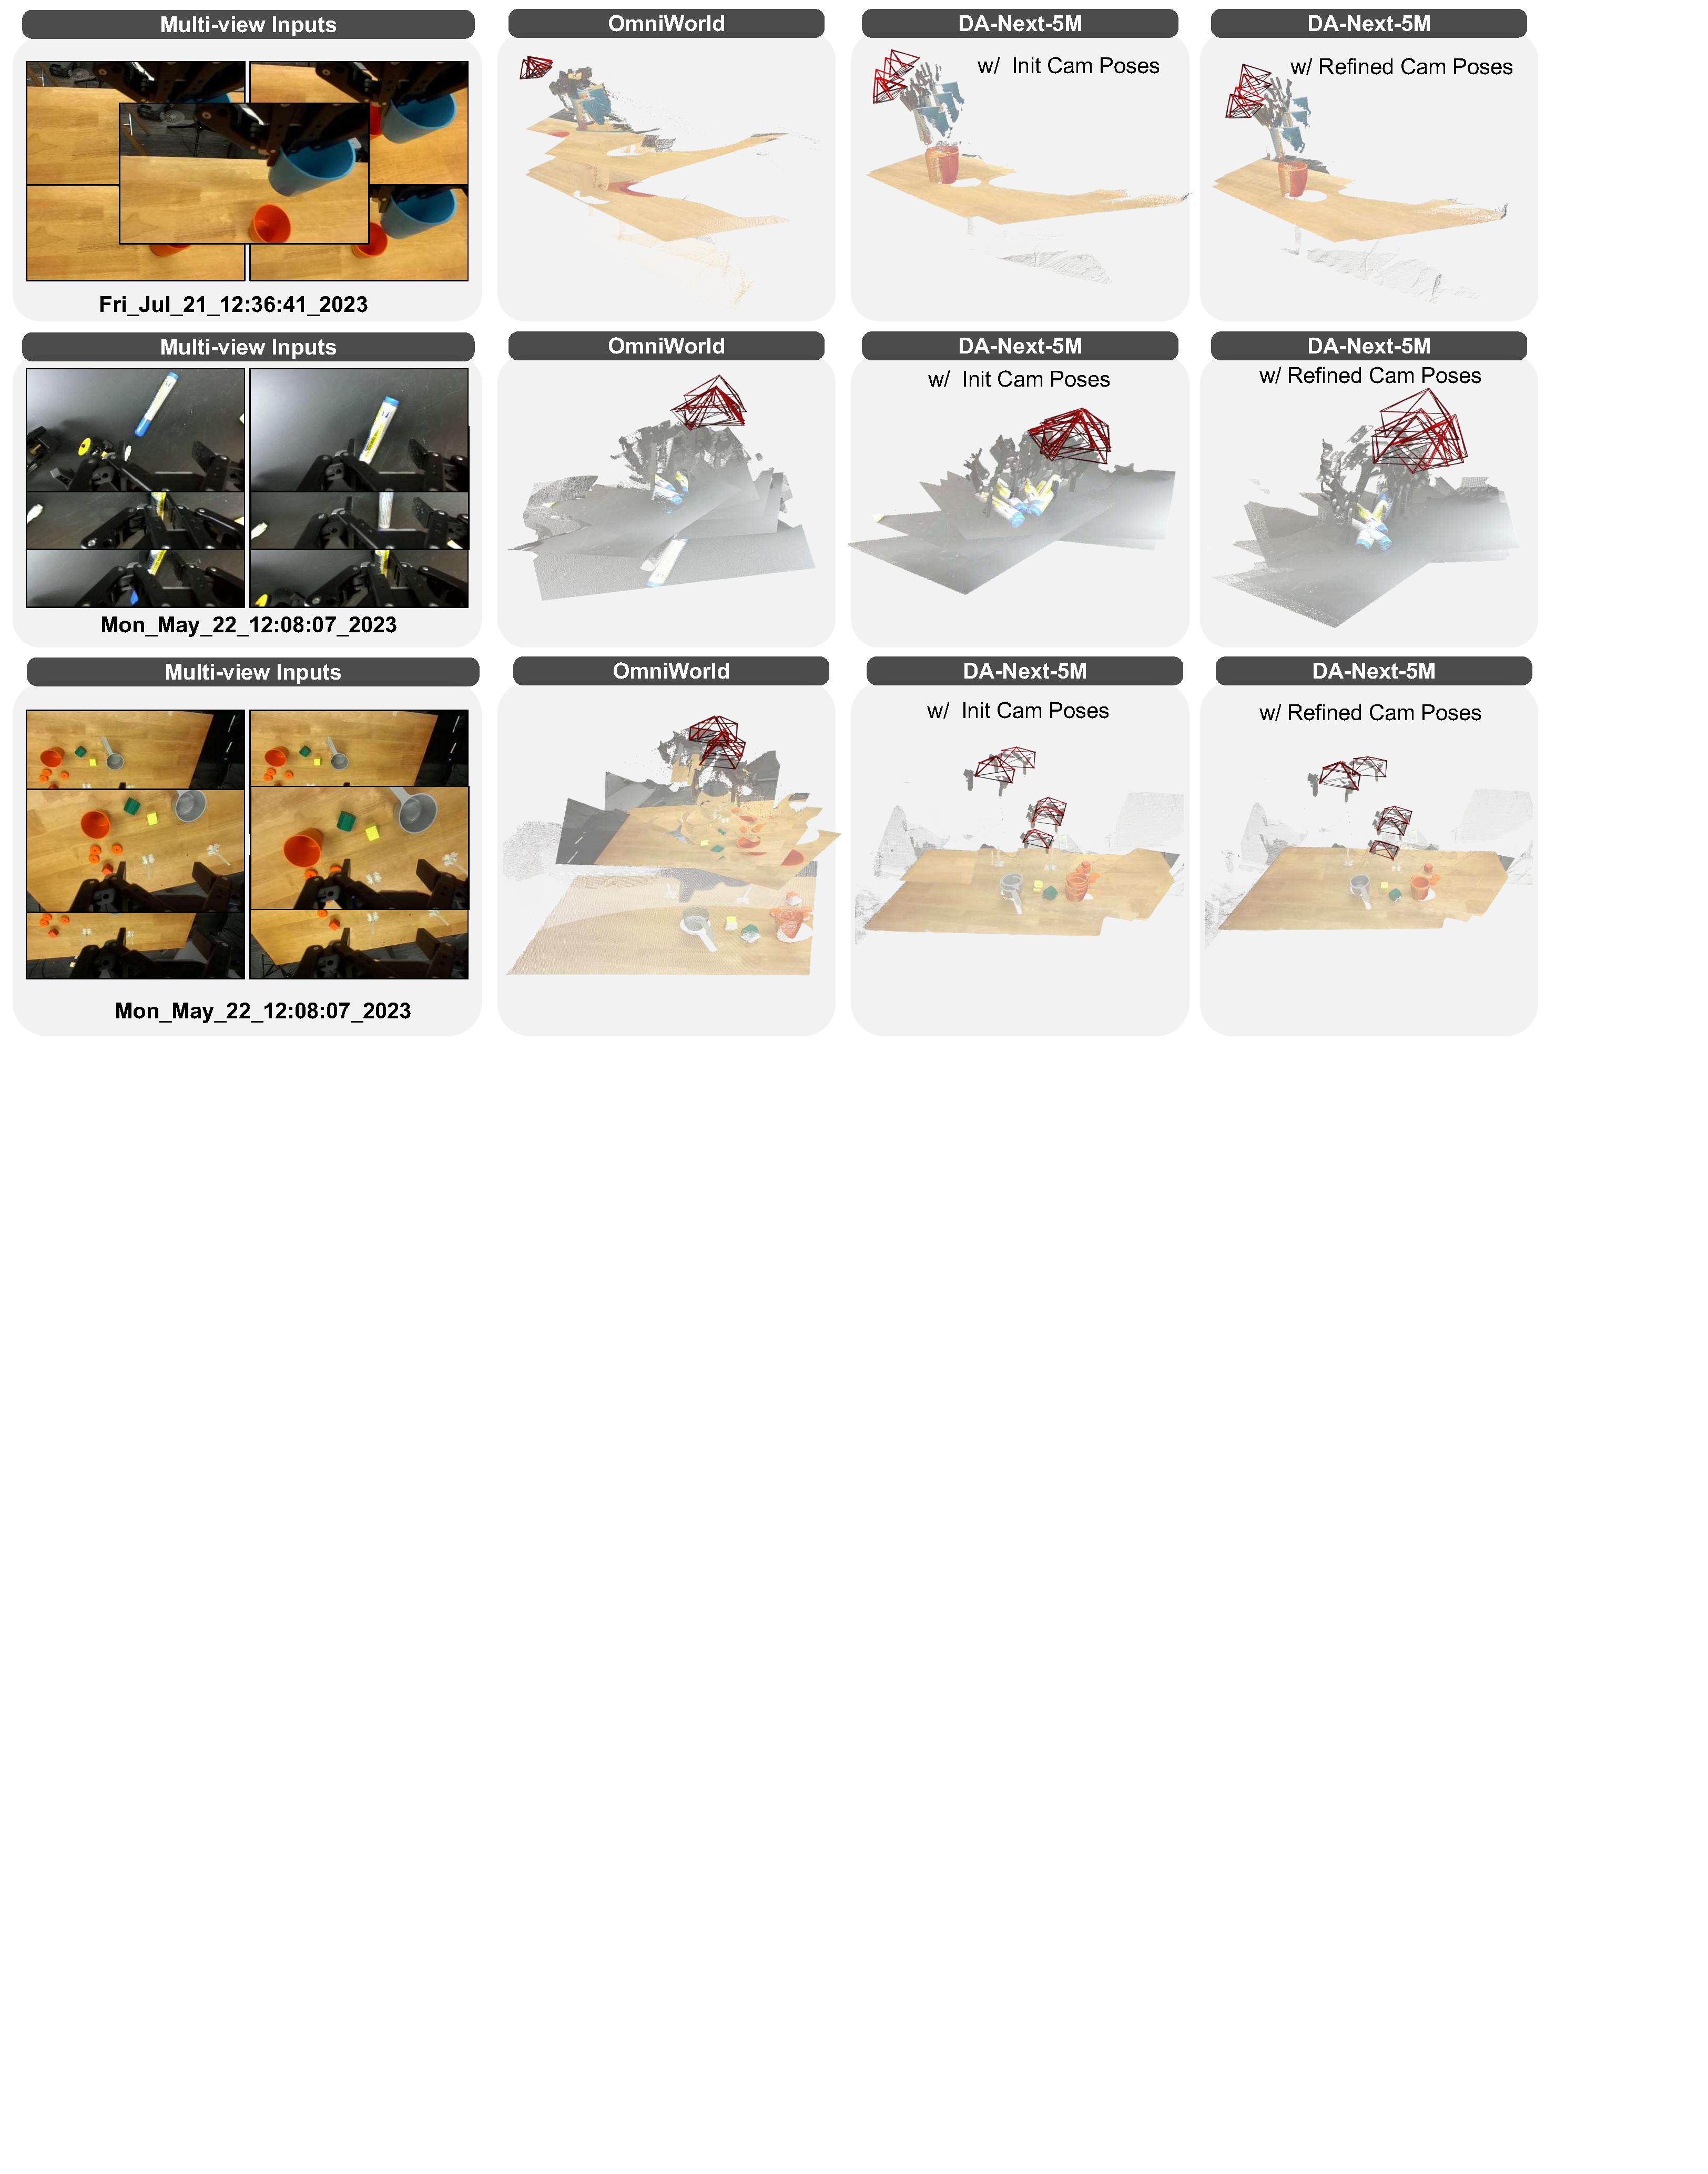
\includegraphics[width=0.9\columnwidth]{figs/droid_vis.pdf}
\caption{\textbf{Visual comparison on the DROID dataset.} We compare the annotations from OmniWorld against our reconstructed point clouds using initial poses and refined poses, respectively.} 
\vspace{-4pt}
\label{Fig.droid_vis} %
\end{figure}

In this section, we detail the data processing pipeline in \benchmark, covering the post-processing pipelines for Xperience (Sec.~\ref{appendix:ropedia}), DROID (Sec.~\ref{appendix:droid}), and our collected simulation datasets (Sec.~\ref{appendix:other_collection}), as well as a unified depth map post-processing pipeline (Sec.~\ref{appendix:DepthPost-Processing}) applied to selected datasets to ensure annotation quality.


\subsection{DROID Curation Pipeline}
\label{appendix:droid}
%
Accurate geometric annotations are critical for reliable benchmark evaluation.
%
However, the raw DROID~\citep{khazatsky2024droid} data is highly noisy with 
unreliable camera calibration, precluding direct use of the original annotations.
%
We first investigate learning-based annotation solutions, including Mega-SaM~\citep{li2025megasam} and VIPE~\citep{huang2025vipe} for visual SLAM, and Camera Depth Model~\citep{liu2025cdm}, PriorDA~\citep{wang2025priorda}, Lingbot-Depth~\citep{lingbot-depth2026}, and PromptDA~\citep{lin2024promptda} for depth completion. However, none of these methods are trained on wrist-view domains, and we observe significant failure cases under the close-range, high-motion conditions characteristic of this setting.

Since DROID provides synchronized stereo pairs, we turn to stereo-based depth estimation as a more reliable annotation source. 
%
We test S$^2$M$^2$~\citep{min2025s2m2}, FoundationStereo~\citep{wen2025foundationstereo}, IGEV~\citep{xu2025igev++}, DynamicStereo~\citep{Karaev_2023_dynamic_stereo}, and WAFT-Stereo~\citep{wang2026waftstereo}, ultimately selecting S$^2$M$^2$ for its superior performance on wrist-view sequences.
%
Specifically, we randomly select a subset of DROID sequences and feed the left-right stereo image pairs from each wrist-view sequence into S$^2$M$^2$ to obtain disparity maps. 
%
Metric depth maps for the left eye are then computed using the ZED camera intrinsics and baseline, with a confidence threshold of 0.999 applied to mask out unreliable depth predictions.
%
The masked depth maps and camera intrinsics are subsequently injected as priors into MapAnything~\citep{keetha2026mapanything} to obtain initial camera poses.
%
We then employ SAM3~\citep{carion2025sam3} to annotate masks for moving objects on selected keyframes, which are propagated to the full sequence.
%
Finally, leveraging the initial camera poses, RGB images, and propagated masks, we perform Bundle Adjustment with both depth and photometric losses to refine the camera parameters and obtain globally aligned point clouds.
%
Sequences with poor temporal depth consistency are filtered out by computing the mean per-pixel reprojection depth error between adjacent frames.
%
Fig.~\ref{Fig.droid_vis} presents a comparison between our DROID data curation pipeline 
and the OmniWorld data processing approach.
%
OmniWorld annotates wrist-view depth using FoundationStereo and relies on the dataset's original inaccurate camera poses, resulting in unreliable depth estimates and misaligned point clouds across frames (\emph{e.g.}, incorrect depth on the marker pen on the table in \texttt{Mon\_May\_22\_12:08:07\_2023}).
%
In contrast, our annotation pipeline produces temporally consistent depth estimates with well-preserved cross-frame continuity.

We also provide a gallery of the DROID~\citep{khazatsky2024droid} dataset we processed in Fig.~\ref{Fig.droid_gallery1} and \ref{Fig.droid_gallery2}.
%
For each scene, we visualize the first frame of the RGB sequence overlaid with the SAM3 segmentation mask (top-left), the corresponding depth map (bottom-left), and the reconstructed point cloud (right).

\begin{figure}[t] 
\centering 
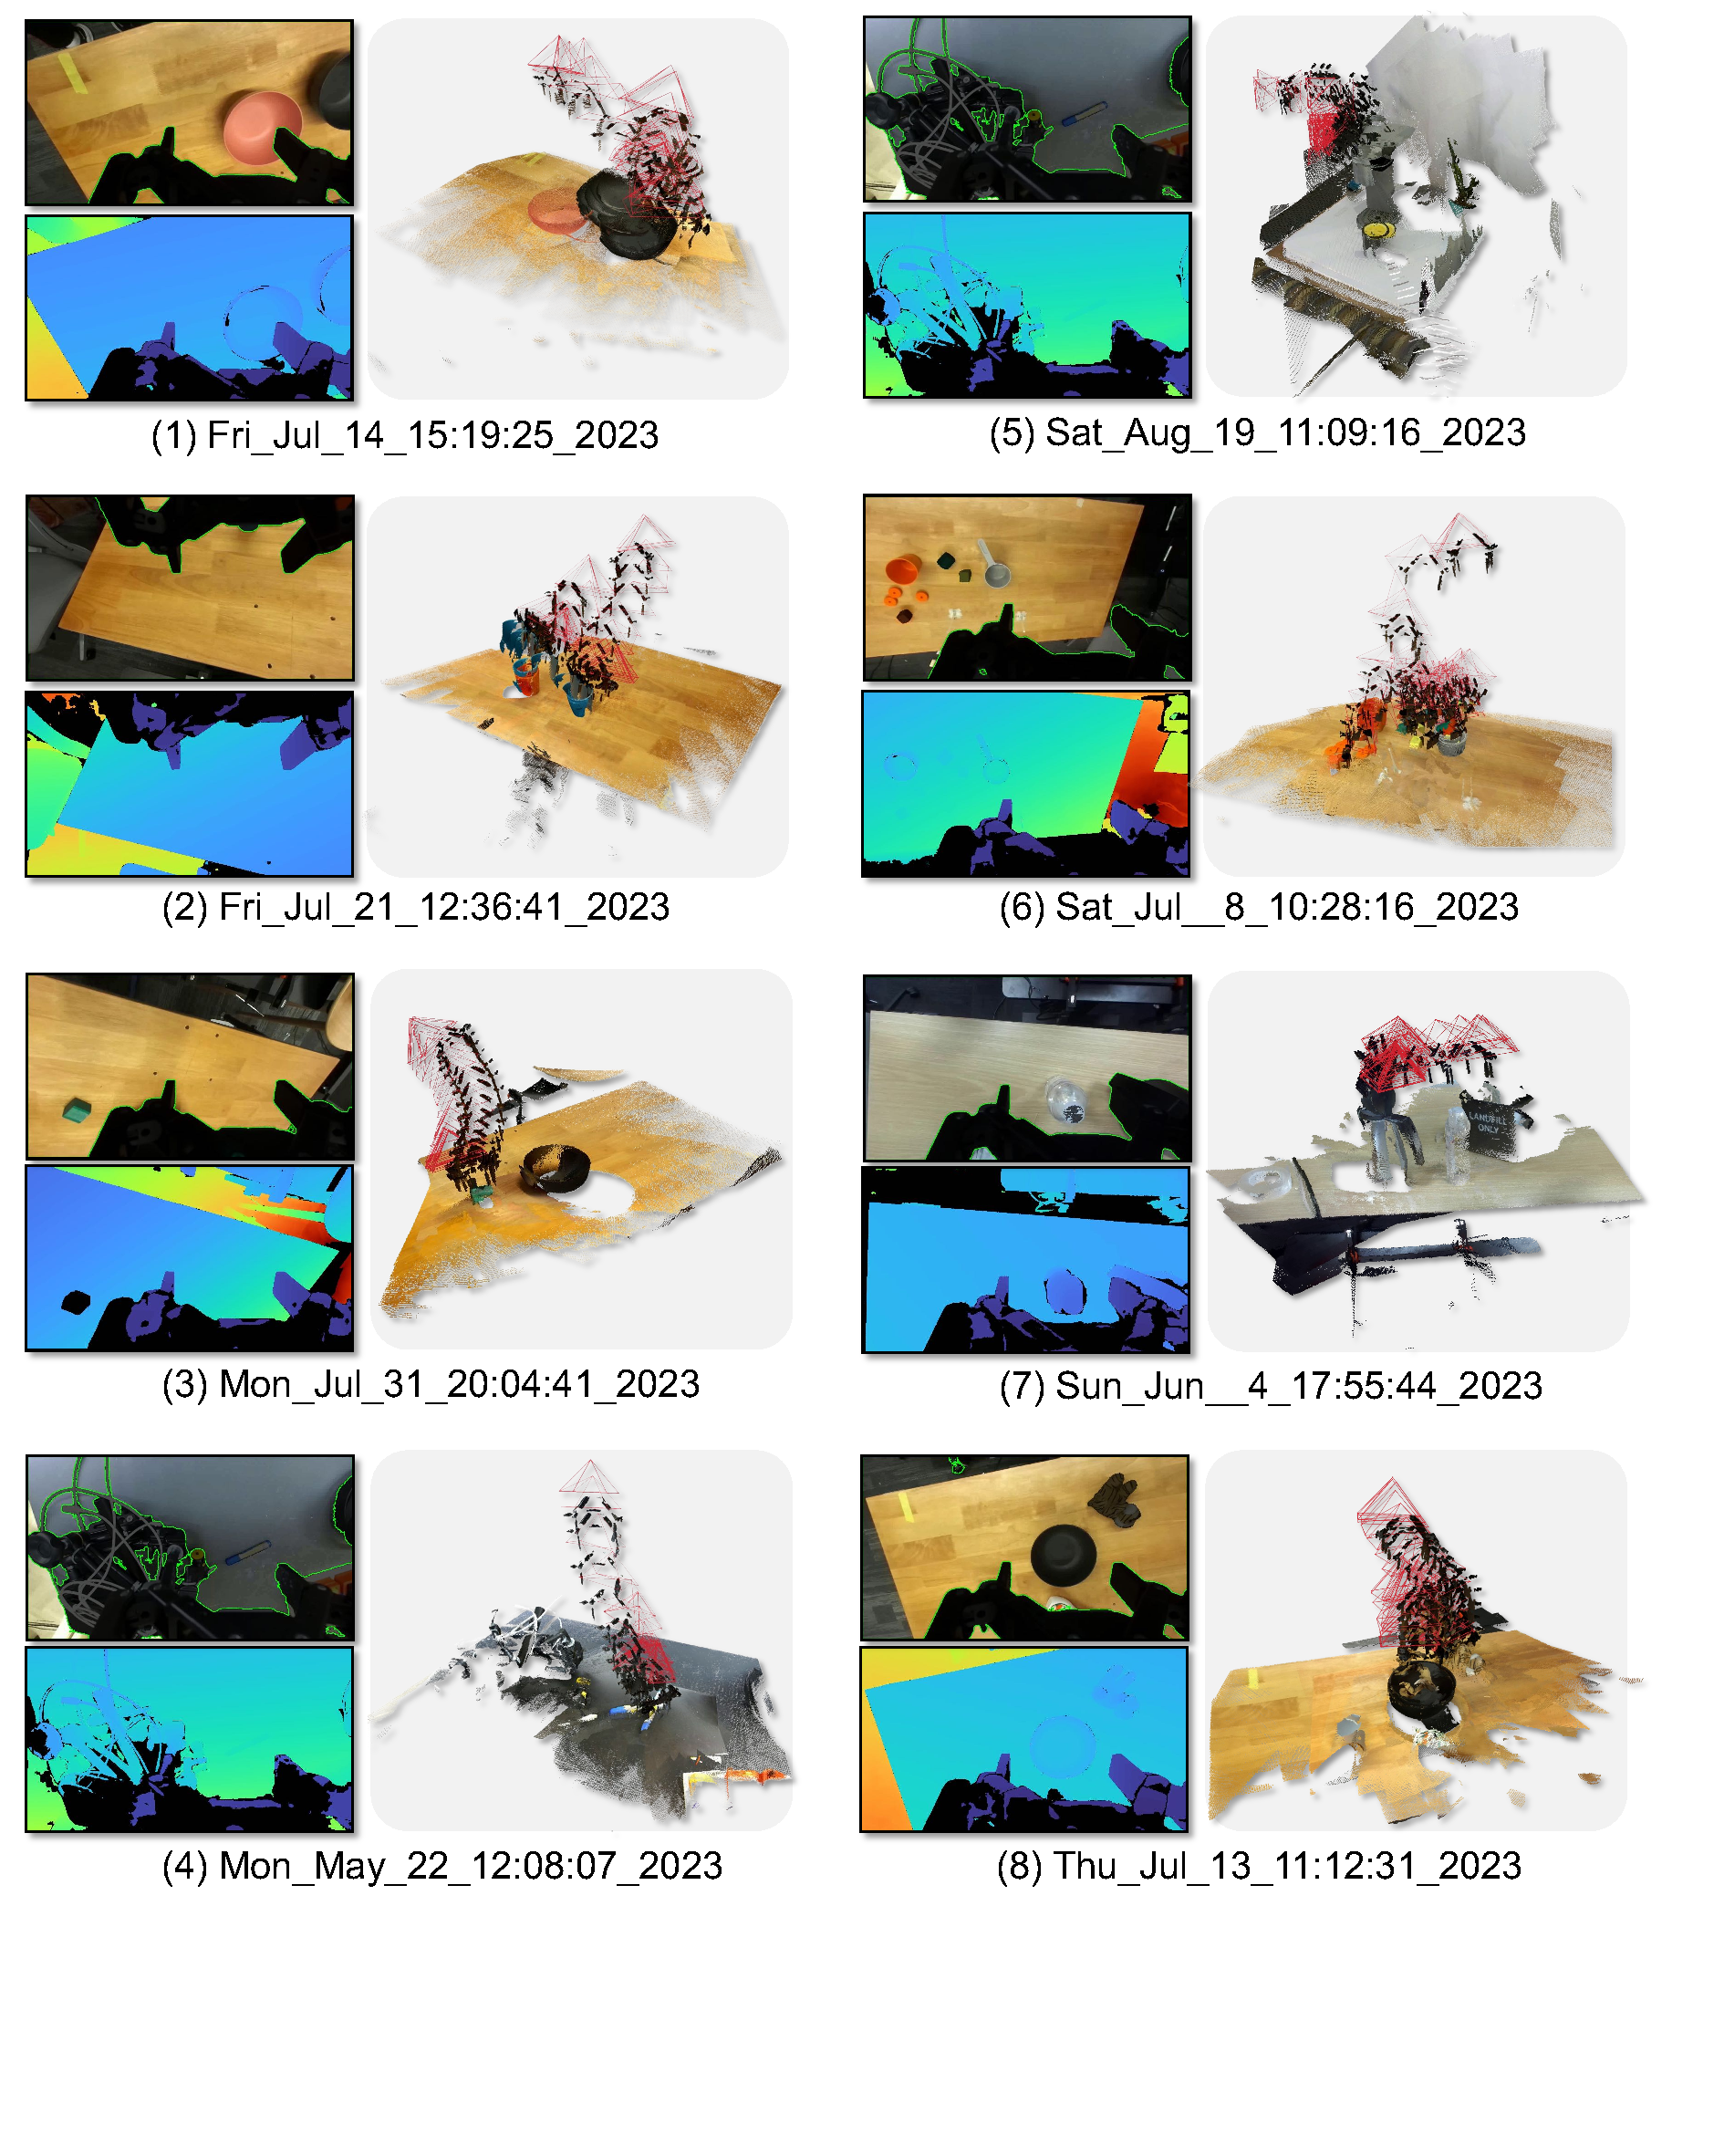
\includegraphics[width=0.9\columnwidth]{figs/droid_gallery1.pdf}
\caption{\textbf{DROID Gallery 1.}} 
\vspace{-4pt}
\label{Fig.droid_gallery1} %
\end{figure}

\begin{figure}[t] 
\centering 
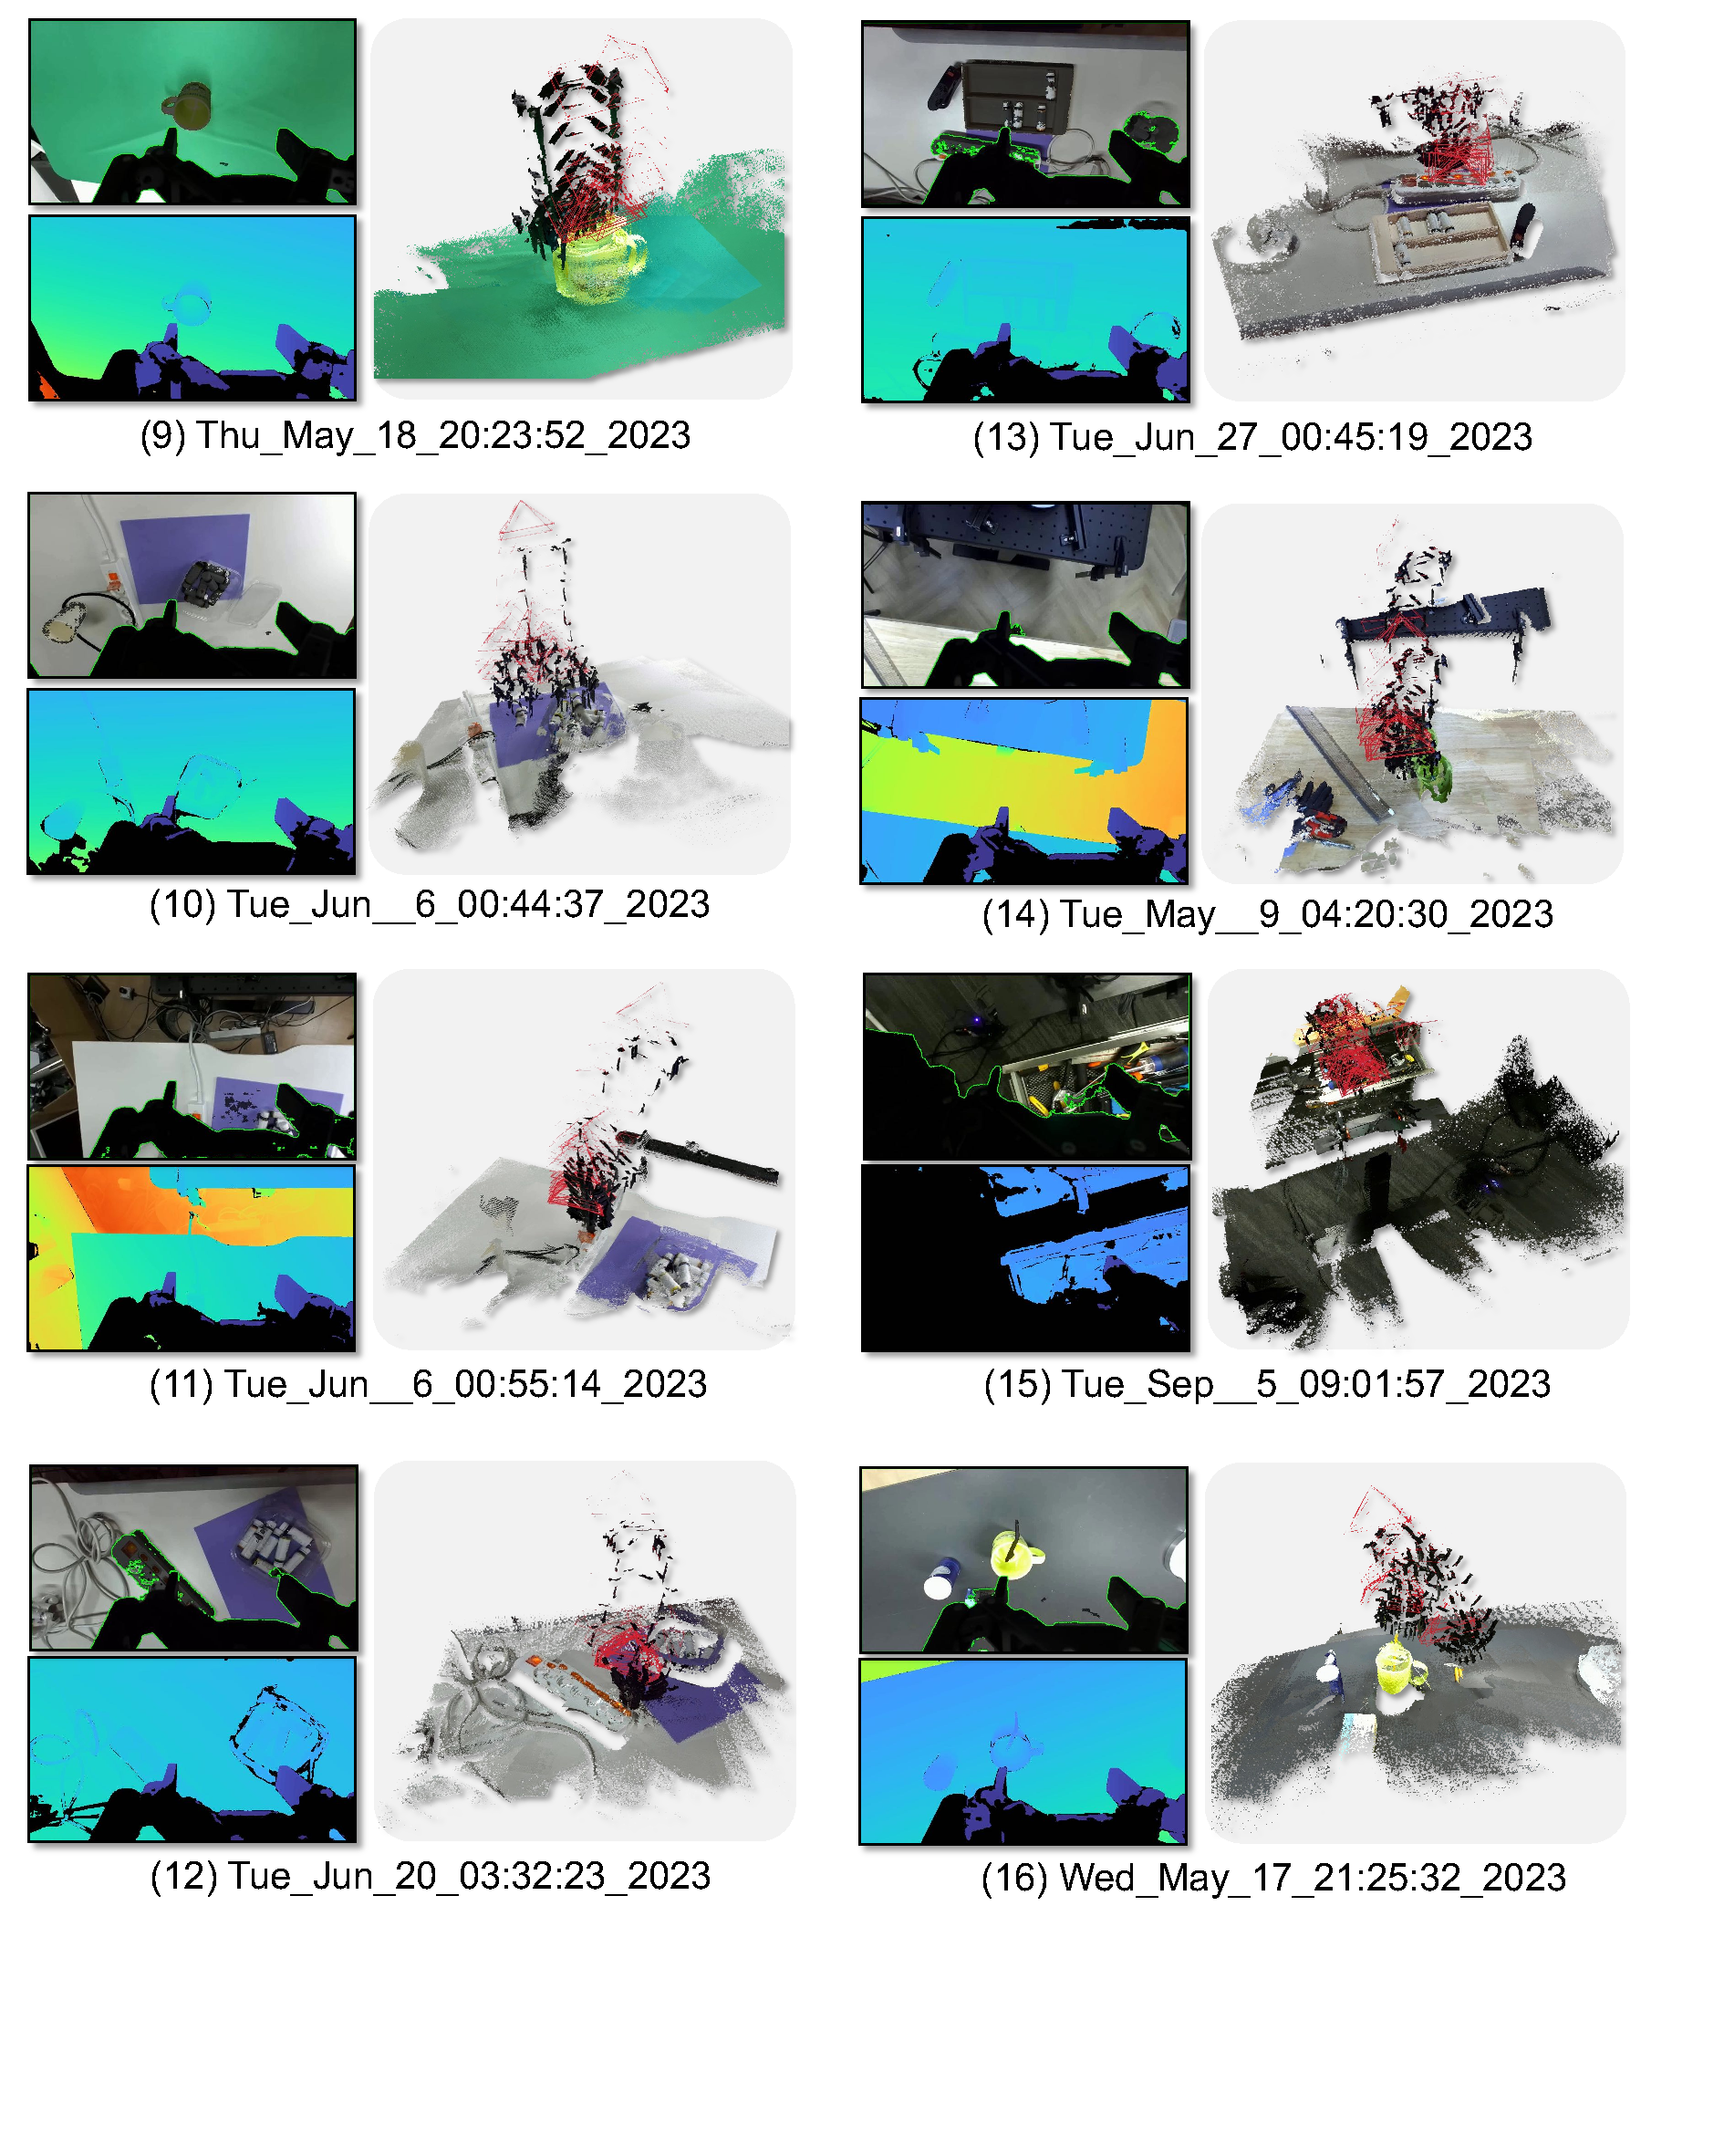
\includegraphics[width=0.9\columnwidth]{figs/droid_gallery2.pdf}
\caption{\textbf{DROID Gallery 2.} } 
\vspace{-4pt}
\label{Fig.droid_gallery2} %
\end{figure}

\subsection{Xperience Curation Pipeline}
\label{appendix:ropedia}
Xperience~\citep{xperience_10m} consists of egocentric sequences captured via a head-mounted device during human activity, recorded by four fisheye cameras.
%
We randomly sample a subset of the original data for processing.
%
We obtain camera poses using a SLAM system built upon VIPE~\citep{huang2025vipe}, and estimate metric depth maps and their confidence maps from rectified stereo image pairs using FoundationStereo~\citep{wen2025foundationstereo}.
%
Fig.~\ref{fig:ropedia_vis} presents sample visualizations of Xperience sequences included 
in \benchmark.

\begin{figure*}
    \centering
    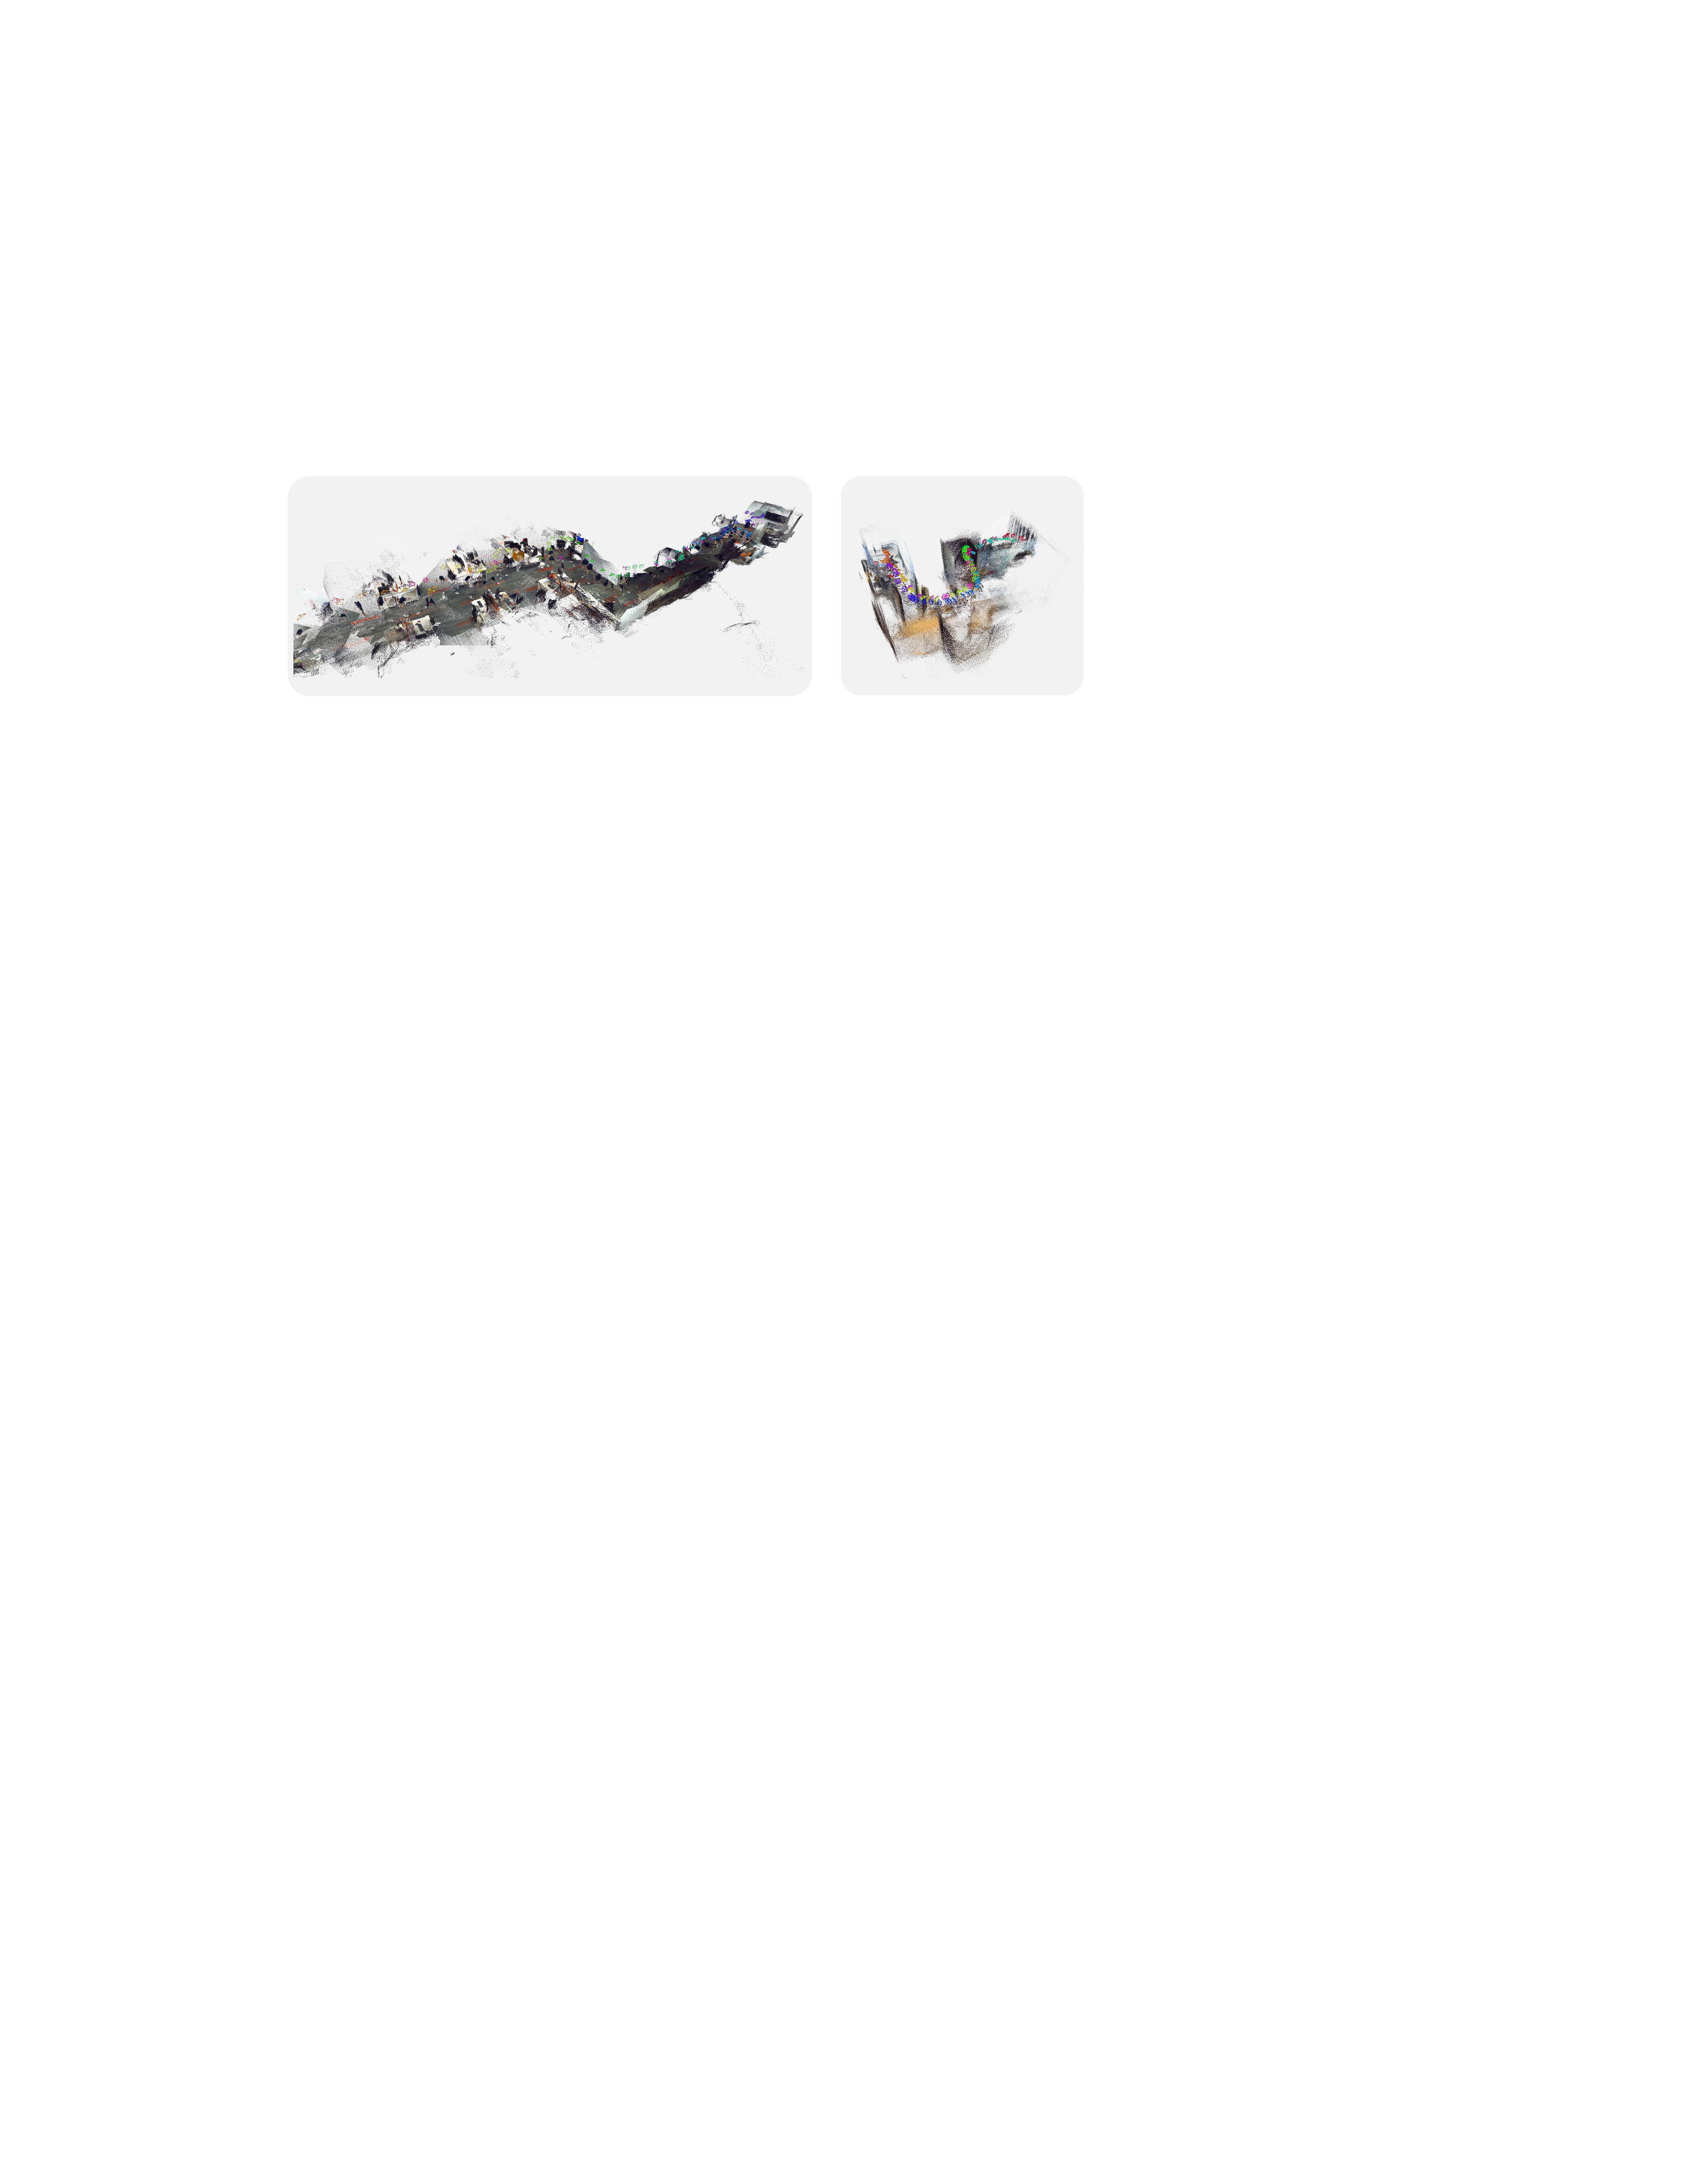
\includegraphics[width=1\linewidth]{figs/ropedia_vis.pdf}
    \caption{\textbf{Visualization of Xperience Samples.} 
}
    \label{fig:ropedia_vis}
    \vspace{-4pt}
\end{figure*}


\subsection{Other Data Collection}
\label{appendix:other_collection}
We collect robot manipulation sequences from four simulators: RLBench~\citep{james2020rlbench}, Robo Colosseum~\citep{pumacay2024colosseum}, RoboTwin~\citep{chen2025robotwin}, and RoboLab~\citep{yang2026robolab}.
%
We refer the reader to Sec.~\ref{appendix:datasets} for details on the data collection procedure.


\subsection{Depth Map Post-Processing Pipeline}
\label{appendix:DepthPost-Processing}
Raw depth maps collected from sensors or simulation engines often contain systematic artifacts that degrade geometric evaluation quality. 
%
We apply a unified five-stage cleaning pipeline to all real-world datasets in \benchmark, producing a per-frame binary validity mask that downstream evaluation uses to ignore unreliable pixels.

\textbf{Stage 1: Depth Range Clipping.}
Depth values are first converted to meters and then clipped to a scene-appropriate valid range $[d_{\min}, d_{\max}]$. 
%
Pixels falling outside this range, including near-field sensor noise and far-field sensor dropout are marked invalid.
%
The range bounds are set per dataset according to the typical operating distance of the capture platform (\emph{e.g.}, $[0.05\text{m},\,5\text{m}]$ for egocentric indoor scenes and $[0\text{m},\,3\text{m}]$ for close-range wrist-view sequences).

\textbf{Stage 2: Flying Point Removal.}
Flying points are erroneous depth values that appear at depth discontinuity boundaries, caused by stereo mismatches or sensor mixed-pixel effects.
%
We detect them by computing the spatial gradient of the depth map and identifying pixels where the gradient magnitude is disproportionately large relative to the local depth value, which indicates a sharp, physically implausible depth jump.
%
Detected discontinuity pixels and a small surrounding neighborhood (controlled by an erosion radius) are masked out, preventing boundary artifacts from contaminating geometric metrics.

\textbf{Stage 3: Edge-Aware Bilateral Filtering.}
Surviving valid pixels are smoothed using a joint bilateral filter guided by the corresponding RGB image.
%
The filter suppresses high-frequency depth noise while preserving genuine depth edges aligned with visible object boundaries.
%
Only already-valid pixels are updated; no hole-filling is performed, ensuring that masked regions remain invalid after filtering.

\textbf{Stage 4: Small Isolated Region Removal.}
After filtering, the valid-pixel mask may contain small, disconnected clusters of surviving pixels that are physically implausible as independent surface patches.
%
We apply connected-component analysis on the binary valid mask and remove any component whose area falls below a minimum threshold, eliminating residual noise fragments that escaped the earlier stages.

\textbf{Stage 5: Sky Mask.}
For outdoor datasets (\emph{e.g.}, OmniWorld~\citep{zhou2025omniworld}, Lingbot-Depth~\citep{lingbot-depth2026}), depth sensors and stereo algorithms systematically fail on sky regions, producing either missing values or extreme outliers at near-infinite range. 
%
We generate a per-frame sky mask using a pretrained semantic segmentation model (SegFormer~\citep{xie2021segformer} fine-tuned on ADE20K~\citep{zhou2019ade20k}) and set all sky-classified pixels to invalid regardless of their depth values.
%
This prevents sky regions from inflating depth error metrics or introducing spurious points at the horizon in point cloud evaluation.
